

\tikzset{every picture/.style={line width=0.75pt}} %set default line width to 0.75pt        

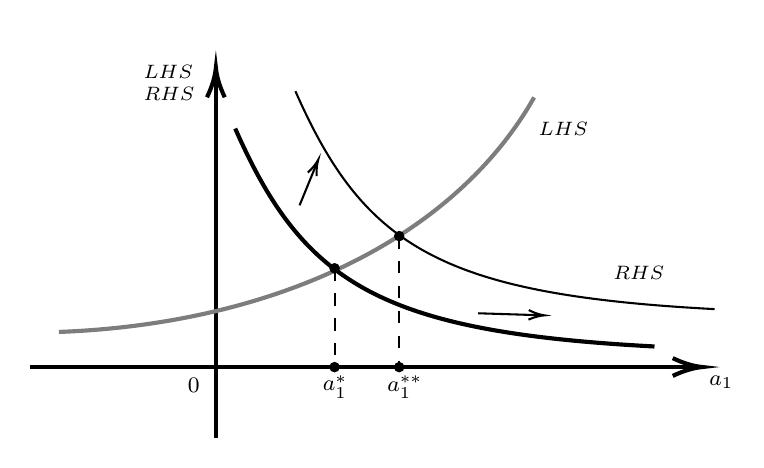
\begin{tikzpicture}[x=0.75pt,y=0.75pt,yscale=-1,xscale=1]
%uncomment if require: \path (0,326); %set diagram left start at 0, and has height of 326

%Straight Lines [id:da021480241971143954] 
\draw [line width=1.5]    (116.33,254) -- (437.33,254) ;
\draw [shift={(440.33,254)}, rotate = 180] [color={rgb, 255:red, 0; green, 0; blue, 0 }  ][line width=1.5]    (14.21,-4.28) .. controls (9.04,-1.82) and (4.3,-0.39) .. (0,0) .. controls (4.3,0.39) and (9.04,1.82) .. (14.21,4.28)   ;
%Straight Lines [id:da6002628265657737] 
\draw [line width=1.5]    (206,288) -- (206,112.83) ;
\draw [shift={(206,109.83)}, rotate = 90] [color={rgb, 255:red, 0; green, 0; blue, 0 }  ][line width=1.5]    (14.21,-4.28) .. controls (9.04,-1.82) and (4.3,-0.39) .. (0,0) .. controls (4.3,0.39) and (9.04,1.82) .. (14.21,4.28)   ;
%Curve Lines [id:da8375485043995874] 
\draw [color={rgb, 255:red, 125; green, 125; blue, 125 }  ,draw opacity=1 ][line width=1.5]    (130.33,237.1) .. controls (236.33,233.1) and (321.33,191.1) .. (359.33,124.1) ;
%Curve Lines [id:da07368504523055663] 
\draw [color={rgb, 255:red, 0; green, 0; blue, 0 }  ,draw opacity=1 ][line width=1.5]    (215.33,139.1) .. controls (248.33,214.1) and (285.33,237.1) .. (417.33,244.1) ;
%Curve Lines [id:da8118414542962347] 
\draw [color={rgb, 255:red, 0; green, 0; blue, 0 }  ,draw opacity=1 ][line width=0.75]    (244.33,121.1) .. controls (277.33,196.1) and (314.33,219.1) .. (446.33,226.1) ;
%Straight Lines [id:da47477618680387335] 
\draw  [dash pattern={on 4.5pt off 4.5pt}]  (263.19,206.42) -- (263.19,254.05) ;
\draw [shift={(263.19,254.05)}, rotate = 90] [color={rgb, 255:red, 0; green, 0; blue, 0 }  ][fill={rgb, 255:red, 0; green, 0; blue, 0 }  ][line width=0.75]      (0, 0) circle [x radius= 2.01, y radius= 2.01]   ;
\draw [shift={(263.19,206.42)}, rotate = 90] [color={rgb, 255:red, 0; green, 0; blue, 0 }  ][fill={rgb, 255:red, 0; green, 0; blue, 0 }  ][line width=0.75]      (0, 0) circle [x radius= 2.01, y radius= 2.01]   ;
%Straight Lines [id:da5558015631901418] 
\draw  [dash pattern={on 4.5pt off 4.5pt}]  (294.33,190.92) -- (294.33,254.05) ;
\draw [shift={(294.33,254.05)}, rotate = 90] [color={rgb, 255:red, 0; green, 0; blue, 0 }  ][fill={rgb, 255:red, 0; green, 0; blue, 0 }  ][line width=0.75]      (0, 0) circle [x radius= 2.01, y radius= 2.01]   ;
\draw [shift={(294.33,190.92)}, rotate = 90] [color={rgb, 255:red, 0; green, 0; blue, 0 }  ][fill={rgb, 255:red, 0; green, 0; blue, 0 }  ][line width=0.75]      (0, 0) circle [x radius= 2.01, y radius= 2.01]   ;
%Straight Lines [id:da7744716619313732] 
\draw [color={rgb, 255:red, 0; green, 0; blue, 0 }  ,draw opacity=1 ][line width=0.75]    (246.33,176.1) -- (254.58,155.96) ;
\draw [shift={(255.33,154.1)}, rotate = 112.25] [color={rgb, 255:red, 0; green, 0; blue, 0 }  ,draw opacity=1 ][line width=0.75]    (7.65,-2.3) .. controls (4.86,-0.97) and (2.31,-0.21) .. (0,0) .. controls (2.31,0.21) and (4.86,0.98) .. (7.65,2.3)   ;
%Straight Lines [id:da2297142609065137] 
\draw [color={rgb, 255:red, 0; green, 0; blue, 0 }  ,draw opacity=1 ][line width=0.75]    (332.33,228.1) -- (362.33,229.04) ;
\draw [shift={(364.33,229.1)}, rotate = 181.79] [color={rgb, 255:red, 0; green, 0; blue, 0 }  ,draw opacity=1 ][line width=0.75]    (7.65,-2.3) .. controls (4.86,-0.97) and (2.31,-0.21) .. (0,0) .. controls (2.31,0.21) and (4.86,0.98) .. (7.65,2.3)   ;

% Text Node
\draw (133,91) node [anchor=north west][inner sep=0.75pt]  [font=\footnotesize] [align=left] {$ $};
% Text Node
\draw (442.33,257) node [anchor=north west][inner sep=0.75pt]  [font=\footnotesize] [align=left] {$a_{1}$};
% Text Node
\draw (163,106.14) node [anchor=north west][inner sep=0.75pt]  [font=\scriptsize] [align=left] {$ \begin{array}{l}
LHS\\
RHS
\end{array}$};
% Text Node
\draw (256,256.49) node [anchor=north west][inner sep=0.75pt]  [font=\footnotesize] [align=left] {$a_{1}^{*}$};
% Text Node
\draw (287.14,256.68) node [anchor=north west][inner sep=0.75pt]  [font=\footnotesize] [align=left] {$a_{1}^{**}$};
% Text Node
\draw (396,204) node [anchor=north west][inner sep=0.75pt]  [font=\scriptsize,color={rgb, 255:red, 0; green, 0; blue, 0 }  ,opacity=1 ] [align=left] {$RHS$};
% Text Node
\draw (360,134.67) node [anchor=north west][inner sep=0.75pt]  [font=\scriptsize,color={rgb, 255:red, 0; green, ; blue, 0 }  ,opacity=1 ] [align=left] {$LHS$};
% Text Node
\draw (191,257.66) node [anchor=north west][inner sep=0.75pt]  [font=\footnotesize] [align=left] {$0$};


\end{tikzpicture}